\documentclass{article}
%%%%%%%%%%%%%%%%%%%%%%%%%%%%%%%%%%%%%%%%%%%%%%%%%%%%%%
% Math
%%%%%%%%%%%%%%%%%%%%%%%%%%%%%%%%%%%%%%%%%%%%%%%%%%%%%%
\usepackage{amsmath}
\usepackage{amssymb}
\usepackage{amsfonts} %para usar as fontes %matematicas, e pega fontes para \mathbb
\usepackage{amsthm}   %ambientes com teoremas (usar depois de amsmath)
%\usepackage{biblatex}
%\usepackage{natbib}

%%%%%%%%%%%%%%%%%%%%%%%%%%%%%%%%%%%%%%%%%%%%%%%%%%%%%%
%Graphs
%%%%%%%%%%%%%%%%%%%%%%%%%%%%%%%%%%%%%%%%%%%%%%%%%%%%%%
\usepackage{graphics}
\usepackage{graphicx}
\usepackage{texdraw}
\usepackage{color}
\usepackage{subfigure} 
\usepackage{tikz}
\usepackage[usenames,dvipsnames]{pstricks}
\usepackage{epsfig}
%\usepackage{pst-grad} % For gradients
%\usepackage{pst-plot} % For axes
%\usepackage{movie15}
\usepackage{animate}
\usetikzlibrary{decorations.fractals}
\usepackage{tikz}
%\usepackage{wrapfig}
\usepackage{pstricks}
\usepackage{multirow}
%%%%%%%%%%%%%%%%%%%%%%%%%%%%%%%%%%%%%%%%%%%%%%%%%%%%%%
% Format
%%%%%%%%%%%%%%%%%%%%%%%%%%%%%%%%%%%%%%%%%%%%%%%%%%%%%%
\usepackage[figurename=Fig.]{caption}
\usepackage[labelformat=empty]{caption}
\usepackage{gensymb}
\usepackage{cancel}
\usepackage{caption} % removing prefix from figure caption in LaTeX
\usepackage{subcaption}
\usepackage{url}
\usepackage{setspace}
%\usepackage{verbatim}
\usepackage{hyperref}
\usepackage{fancyhdr}
\usepackage{pgf}
%%%%%%%%%%%%%%%%%%%%%%%%%%%%%%%%%%%%%%%%%%%%%%%%%%%%%%
% Graphs path to the Picture Folder
%%%%%%%%%%%%%%%%%%%%%%%%%%%%%%%%%%%%%%%%%%%%%%%%%%%%%%
%\graphicspath{/home/henry/Desktop/UTEP_Proposal_Thesis/PhD_Thesis/Pictures}
\graphicspath{{Pictures/}{Data/}{References}} % Two folders Picture and Data    
%%%%%%%%%%%%%%%%%%%%%%%%%%%%%%%%%%%%%%%%%%%%%%%%%%%%%%
% page edition
%%%%%%%%%%%%%%%%%%%%%%%%%%%%%%%%%%%%%%%%%%%%%%%%%%%%%%
%\linespread{2.5}
\addtolength{\textwidth}{3cm}
\addtolength{\textheight}{3cm}
\addtolength{\hoffset}{-2cm}
% In case you need to adjust margins:
\topmargin=-0.5 in      %
\evensidemargin= .5 in     %
\oddsidemargin= .5 in      %
\textwidth = 7 in        %
\textheight = 9.0 in       %
\headsep = 0.15 in  
\pagestyle{fancyplain}
\lhead{\fancyplain{}{ORNL-HPGMG Benchmark-Summer 2017}}
\rhead{\fancyplain{}{Henry R Moncada}}

%%%%%%%%%%%%%%%%%%%%%%%%%%%%%%%%%%%%%%%%%%%%%%%%%%%%%%
% bibliography
%%%%%%%%%%%%%%%%%%%%%%%%%%%%%%%%%%%%%%%%%%%%%%%%%%%%%%
%\usepackage{biblatex}
\bibliographystyle{plain}
%\bibliography{urlbib}

\begin{document}
% \centerline{\sc \large University of Texas at El Paso}
% \centerline{\sc \large Computational Science (CPS) }
% \vspace{1pc}
% \centerline{\sc \Large A short tutorial}
% \vspace{1pc}
% \centerline{\sc \Large ALADDIN Installions}

\title{ University of Texas at El Paso\\
Computational Science\\
PETSC STAMPEDE}
\author{Henry R. Moncada}
\maketitle
\tableofcontents        % Generate Table of Contents


\section{Introduction}
Since \verb+05/18/17+ Stampede 1's KNL sub-system is no longer available, and the KNL material in the Stampede 1 User Guide is now obsolete

\section{QUICK START ON STAMPEDE 2}
\begin{enumerate}
\item Open a terminal and \verb+CD+ to your work forder directory 
\scriptsize
\begin{verbatim}
$ ssh hmoncada@stampede2.tacc.utexas.edu
\end{verbatim}
\normalsize
\item Log into Stampede 
\scriptsize
\begin{verbatim}
henry@Lola:~/Desktop/PETSC/Stampede/SVL$ ssh hmoncada@stampede2.tacc.utexas.edu

To access the system:

1) If not using ssh-keys, please enter your TACC password at the password prompt
2) At the TACC Token prompt, enter your 6-digit code followed by <return>.  

Password: 
SMS Submitted
TACC Token Code:
Last login: Wed Aug 30 12:38:21 2017 from 192.188.177.50
------------------------------------------------------------------------------
                   Welcome to the Stampede2 Supercomputer
      Texas Advanced Computing Center, The University of Texas at Austin
------------------------------------------------------------------------------

              ** Unauthorized use/access is prohibited. **

If you log on to this computer system, you acknowledge your awareness
of and concurrence with the UT Austin Acceptable Use Policy. The
University will prosecute violators to the full extent of the law.

TACC Usage Policies:
http://www.tacc.utexas.edu/user-services/usage-policies/
______________________________________________________________________________

Welcome to Stampede2, *please* read these important system notes:

--> Stampede2 has entered early operations for Phase 1, Phase 2 will be coming
    this fall
--> Stampede2 user documentation is available at:
       https://portal.tacc.utexas.edu/user-guides/stampede2

--------------------- Project balances for user hmoncada ----------------------
| Name           Avail SUs     Expires | Name           Avail SUs     Expires |
| TG-ASC140011        1320  2018-01-03 | TG-DMR160140        1203  2017-10-03 | 
------------------------ Disk quotas for user hmoncada ------------------------
| Disk         Usage (GB)     Limit    %Used   File Usage       Limit   %Used |
| /home1              0.4      10.0     4.08          486      200000    0.24 |
| /work               0.0    1024.0     0.00           17     3000000    0.00 |
| /scratch            0.0       0.0     0.00            6           0    0.00 |
-------------------------------------------------------------------------------

Tip 202   (See "module help tacc_tips" for features or how to disable)

   Did you know that job resource utilization reports are available via TACC's remora tool? Try it:
     $ module load remora
     $ module help remora

login4.stampede2(1)$ 
\end{verbatim}
\normalsize
\item Navegate on your directory and find your SVL-PETSC Folder:
\scriptsize
\begin{verbatim}
login2.stampede$ pwd
/home1/02817/hmoncada/SVL/SVL_V_2_2_PETSC_TACC
\end{verbatim}
\normalsize
\item Clean trash in the Folder:
\scriptsize
\begin{verbatim}
login2.stampede$ vi SVL_Clean.sh
#!/bin/sh
rm OUTPUT_*.mat
rm OUTPUT_*
rm log.txt
rm my_job_err.*
rm my_job_out.*
rm *.o
\end{verbatim}
\normalsize
Execute Clean
\scriptsize
\begin{verbatim}
login2.stampede$ bash SVL_Clean.sh
\end{verbatim}
\normalsize
\item Module loads:
\scriptsize
\begin{verbatim}
login4.stampede2(17)$ module load petsc/3.7-complex
login4.stampede2(18)$ module load fftw3/3.3.6 
login4.stampede2(19)$ module list

Currently Loaded Modules:
  1) intel/17.0.4   2) impi/17.0.3   3) git/2.9.0   4) autotools/1.1   5) python/2.7.13   6) xalt/1.7   7) TACC   8) petsc/3.7-complex   9) fftw3/3.3.6
\end{verbatim}
\normalsize
\end{enumerate}


\section{SVL AT STAMPEDE 2}    
\subsection{Log in}
\begin{enumerate}
\item Open a terminal and \verb+CD+ to your workspace directory. Remember we are now on \verb+Stampede2+, do not forget to type \verb+2+ after \verb+Stampede+ 
\scriptsize
\begin{verbatim}
$ ssh hmoncada@stampede2.tacc.utexas.edu
\end{verbatim}
\normalsize
\item Log into Stampede 
\scriptsize
\begin{verbatim}
henry@Fiona:~/Desktop/PETSC/Examples/SVL_3D_V_2_3_PETSC_DESKTOP$ ssh hmoncada@stampede2.tacc.utexas.edu
The authenticity of host 'stampede2.tacc.utexas.edu (129.114.63.44)' can't be established.
ECDSA key fingerprint is SHA256:SegC2YyyftiRpdwhXqNZE+15RyGeFSal4Vuz0HYJ5E8.
Are you sure you want to continue connecting (yes/no)? yes
Warning: Permanently added 'stampede2.tacc.utexas.edu,129.114.63.44' (ECDSA) to the list of known hosts.

To access the system:

1) If not using ssh-keys, please enter your TACC password at the password prompt
2) At the TACC Token prompt, enter your 6-digit code followed by <return>.  

Password: 
SMS Submitted
TACC Token Code:
Last login: Thu Aug 31 08:39:37 2017 from 192.188.177.50
------------------------------------------------------------------------------
                   Welcome to the Stampede2 Supercomputer
      Texas Advanced Computing Center, The University of Texas at Austin
------------------------------------------------------------------------------

              ** Unauthorized use/access is prohibited. **

If you log on to this computer system, you acknowledge your awareness
of and concurrence with the UT Austin Acceptable Use Policy. The
University will prosecute violators to the full extent of the law.

TACC Usage Policies:
http://www.tacc.utexas.edu/user-services/usage-policies/
______________________________________________________________________________

Welcome to Stampede2, *please* read these important system notes:

--> Stampede2 has entered early operations for Phase 1, Phase 2 will be coming
    this fall
--> Stampede2 user documentation is available at:
       https://portal.tacc.utexas.edu/user-guides/stampede2

--------------------- Project balances for user hmoncada ----------------------
| Name           Avail SUs     Expires | Name           Avail SUs     Expires |
| TG-ASC140011        1320  2018-01-03 | TG-DMR160140        1203  2017-10-03 | 
------------------------ Disk quotas for user hmoncada ------------------------
| Disk         Usage (GB)     Limit    %Used   File Usage       Limit   %Used |
| /home1              0.4      10.0     4.08          498      200000    0.25 |
| /work               0.0    1024.0     0.00           19     3000000    0.00 |
| /scratch            0.0       0.0     0.00            8           0    0.00 |
-------------------------------------------------------------------------------

Tip 56   (See "module help tacc_tips" for features or how to disable)

   Vim supports ctags (a code database.) ctags -R *; Ctrl-] will jump to a function definition underneath the cursor.

login4.stampede2(1)$ ll
\end{verbatim}
\normalsize
\item My \verb+Stampede2+ home directory
\scriptsize
\begin{verbatim}
login1(1001)$ ll
total 9924
drwx------  3 hmoncada G-815332    4096 Aug 31  2017 intel
drwx------  2 hmoncada G-815332    4096 Aug 31  2017 Others
-rw-------  1 hmoncada G-815332 3141431 Apr 13  2018 SKX_OUT_1_2_16_11_5_C2.tar.gz
-rw-------  1 hmoncada G-815332 5187802 Apr 13  2018 SKX_OUT_1_2_16_13_5_C2.tar.gz
-rw-------  1 hmoncada G-815332 1813833 Apr 13  2018 SKX_OUT_1_2_16_9_5_C2.tar.gz
drwx------ 11 hmoncada G-815332    4096 Apr 12  2018 SVL_NEW
drwx------ 13 hmoncada G-815332    4096 Sep 18  2017 SVL_OLD
\end{verbatim}
\normalsize
\item Copies the directory \verb+mysrc+ and its contents from your \verb+Stampede1+ home directory to your \verb+Stampede2+ home directory.
\scriptsize
\begin{verbatim}
login4.stampede2(1)$ cp -r $OLDHOME/mysrc $HOME/
\end{verbatim}
\normalsize
where \verb+mysrc+ is the name of the directory you wish to move. For example, I wish to move \verb+SVL+ to \verb+Stampede2+ with a new name \verb+SVL_OLD+
\scriptsize
\begin{verbatim}
login4.stampede2(1)$ cp -r $OLDHOME/SVL $HOME/SVL_OLD
\end{verbatim}
\normalsize
\scriptsize
\begin{verbatim}
login1.stampede2(20)$ ll
total 16
drwx------  3 hmoncada G-815332 4096 Aug 31 11:09 intel
drwx------  2 hmoncada G-815332 4096 Aug 31 08:41 Others
drwx------ 13 hmoncada G-815332 4096 Aug 30 13:57 SVL_NEW
drwx------ 13 hmoncada G-815332 4096 Sep 18 13:11 SVL_OLD
\end{verbatim}
\normalsize
\item \verb+CD+ to \verb+SVL_OLD+
\scriptsize
\begin{verbatim}
login1.stampede2(23)$ cd SVL_OLD/
login1.stampede2(24)$ ll
total 44
drwx------ 2 hmoncada G-815332 4096 Sep 18 13:11 example_8_FFTW
drwx------ 2 hmoncada G-815332 4096 Sep 18 13:11 FDDER
drwx------ 4 hmoncada G-815332 4096 Sep 18 13:11 fftw_mpi
drwx------ 2 hmoncada G-815332 4096 Sep 18 13:11 SVL_01_PETSC_Compile_Multiple_C_Files_in_a_Program
drwx------ 5 hmoncada G-815332 4096 Sep 18 13:11 SVL_3D_V_3_2_PETSC_TACC
drwx------ 2 hmoncada G-815332 4096 Sep 18 13:11 SVL_3D_V_3_3_PETSC_TACC
drwx------ 2 hmoncada G-815332 4096 Sep 18 13:11 SVL_CSparse_Compile_Multiple_C_Files_in_a_Program
drwx------ 2 hmoncada G-815332 4096 Sep 18 13:11 SVL_Project
drwx------ 2 hmoncada G-815332 4096 Sep 18 13:11 SVL_V_2_1_PETSC_TACC
drwx------ 2 hmoncada G-815332 4096 Sep 18 13:11 SVL_V_2_2_PETSC_TACC
drwx------ 2 hmoncada G-815332 4096 Sep 18 13:11 SVL_V_3_1_PETSC_TACC
\end{verbatim}
\normalsize
\item \verb+CD+ to \verb+SVL_NEW+
\scriptsize
\begin{verbatim}
login1(1003)$ cd SVL_NEW/
login1(1004)$ ll
total 140
drwx------  3 hmoncada G-815332 16384 Apr 12  2018 KNL_SVL_3D_PETSCSCALAR_MAR_13_2018
drwx------  5 hmoncada G-815332 12288 Apr 12  2018 SKX_SVL_3D_PETSCSCALAR_MAR_13_2018
drwx------ 11 hmoncada G-815332  4096 Feb 16  2018 SVL_2D
drwx------ 14 hmoncada G-815332  4096 Mar 13  2018 SVL_3D_OLD
drwx------  2 hmoncada G-815332 32768 Apr 18  2018 SVL_3D_PETSCSCALAR_COMPLEX_TACC_Feb_21_2018
drwx------  5 hmoncada G-815332 12288 Apr  2  2018 SVL_3D_PETSCSCALAR_MALLOC
drwx------  2 hmoncada G-815332 12288 Apr 12  2018 TAU_KNL_SVL_3D_PETSCSCALAR
-rw-------  1 hmoncada G-815332 10260 Apr 12  2018 TAU_KNL.tar.gz
drwx------  2 hmoncada G-815332 12288 Apr 12  2018 TAU_SKX_SVL_3D_PETSCSCALAR
-rw-------  1 hmoncada G-815332 10226 Apr 12  2018 TAU_SKX.tar.gz
drwx------  5 hmoncada G-815332 12288 Apr 12  2018 TAU_SVL_3D_PETSCSCALAR_MAR_13_2018
\end{verbatim}
\normalsize
\end{enumerate}

\subsection{Makefile}
Before compile and submit any code on \verb+stampede2+. We need to made few modification into the  \verb+Makefile+ in order to made it work.
\begin{enumerate}
\item \verb+CD+ into one of your code folders, like the following for example \verb+SVL_V_3_1_PETSC_TAC+
\item Module loads
\scriptsize
\begin{verbatim}
login1.stampede2(44)$ module load fftw3
login1.stampede2(45)$ module load petsc/3.7-complex
login1.stampede2(67)$ module load matlab
login1.stampede2(68)$ module list

Currently Loaded Modules:
  1) intel/17.0.4   2) impi/17.0.3   3) git/2.9.0   4) autotools/1.1   5) python/2.7.13   6) xalt/1.7   7) TACC   8) petsc/3.7-complex   9) fftw3/3.3.6  10) matlab/2017a

\end{verbatim}
\normalsize
\item The SVL code require a few tools such as \verb+FFTW+.  
We need to specify the search path directories. The search path directories are usually added with the options (flat) \verb+-I+ and \verb+-L+.
These option flat will link our \verb+SVL+ code to the require libraries. The path directories are found using the \verb+echo+ comnmand on the \verb+STAMPEDE2+ terminal.
\scriptsize
\begin{verbatim}
login1.stampede2(49)$ echo $TACC_FFTW3_INC
/opt/apps/intel17/impi17_0/fftw3/3.3.6/include

login1.stampede2(47)$ echo $TACC_FFTW3_LIB
/opt/apps/intel17/impi17_0/fftw3/3.3.6/lib

login1.stampede2(48)$ echo $TACC_PETSC_LIB
/home1/apps/intel17/impi17_0/petsc/3.7/knightslanding-complex/lib
\end{verbatim}
\normalsize
\item Pase the search paths on the Makefile. Use the option (flap) \verb+-L+  for library and \verb+-I+ for include. 
\item MAKEFILE
\scriptsize
\begin{verbatim}
login2.stampede(38)$ vi Makefile 
CFLAGS           = -I/opt/apps/intel17/impi17_0/fftw3/3.3.6/include
FFLAGS           =
CPPFLAGS         =
FPPFLAGS         =
LOCDIR           =                                      # Working folder
EXAMPLESC        =                                      # *.c or *.cpp file names here
EXAMPLESF        =
MANSEC           =
FFTW_LIBS        = -L/opt/apps/intel17/impi17_0/fftw3/3.3.6/lib -lfftw3     -L\${TACC_FFTW3_LIB} # fftw serial libraries
FFTW_MPI         = -L/opt/apps/intel17/impi17_0/fftw3/3.3.6/lib -lfftw3_mpi -lfftw3 -L\${TACC_FFTW3_LIB} # fftw mpi libraries
MPI_LIBS         = -L\${TACC_MPIP_LIB} -lmpiP     # mpip librarie no longer on stampede2
MATH_lIBS        = -lm        # math libraries
TRASH            :=  *.*~  *~  *.o

SOURCE_PETSC     := SVL_PETSC_3D_DFT_MAIN_ORNL.c\
                    SVL_PETSC_3D_UNIT_CELL_ARRAY.c\
                    SVL_PETSC_3D_ZERO_CELL.c\
                    SVL_PETSC_3D_UNIT_CELL.c\
                    SVL_PETSC_3D_FFTW_SWAP_METHOD_2.c\
                    SVL_PETSC_3D_FFTW.c\
                    SVL_PETSC_3D_SWAP_QUADRANTS.c\
                    SVL_PETSC_3D_IFFTW.c\
                    SVL_PETSC_3D_TRUNCTED_FFTW_ARRAY.c\
                    SVL_PETSC_3D_GRADING_VECTOR.c\
                    SVL_PETSC_3D_IMPLEMENT_IMPROVEMENTS.c\
                    SVL_PETSC_3D_ELIMINATE_GRATING_ACCORD_THEIR_AMPLITUD.c\
                    SVL_PETSC_3D_IDENTIFIED_COLLINEAR_PLANAR_GRATING.c\
                    SVL_PETSC_3D_IMPLEMENT_ATTRIBUTES.c\
                    SVL_PETSC_3D_ORIENTATION_FUNCTION.c\
                    SVL_PETSC_3D_LATTICE_SPACING_FUNCTION.c\
                    SVL_PETSC_3D_IMPROVEMENTS.c\
                    SVL_PETSC_3D_FDDER.c\
                    SVL_PETSC_3D_LOOP.c\
                    SVL_PETSC_3D_ORIENTATION_VECTOR.c\
                    SVL_PETSC_3D_CARTESIAN_TO_SPHERICAL.c\
                    SVL_PETSC_3D_ROTATION.c\
                    SVL_PETSC_3D_SPACING.c\
                    SVL_PETSC_3D_SPHERICAL_TO_CARTESIAN.c\
                    SVL_PETSC_3D_RHS.c\
                    SAVE_1D_TO_3D_ARRAY_REAL.c\
                    SAVE_1D_TO_3D_ARRAY_COMPLEX.c\
                    #SAVE_1D_To_3D_ARRAY_SLIDE.c\
                    #SVL_PETSC_3D_DFT_FFTW_SWAP_ORNL.c\
                    #SVL_PETSC_3D_FFTW_SWAP_METHOD_1.c\
                    #SVL_PETSC_1D_FFTW_X_AXIS.c\
                    #SVL_PETSC_1D_FFTW_Y_AXIS.c\
                    #SVL_PETSC_1D_FFTW_Z_AXIS.c\
                    #SVL_PETSC_1D_SWAP_X_AXIS.c\
                    #SVL_PETSC_1D_SWAP_Y_AXIS.c\
                    #SVL_PETSC_1D_SWAP_Z_AXIS.c\
                    #SVL_PETSC_3D_TRUNCTED_FFTW_SPATIAL_HARMONICS.c\

OBJECTS_PETSC    := $(SOURCE_PETSC:.c=.o)
EXECUTABLE_PETSC := OUTPUT_PETSC

# Version 3.7: These Makefiles lines must be updated every time you Update your petsc version.
include ${PETSC_DIR}/lib/petsc/conf/variables
include ${PETSC_DIR}/lib/petsc/conf/rules

SVL_PETSC: $: $(OBJECTS_PETSC) chkopts
             -${CLINKER} -g -o $(EXECUTABLE_PETSC) $(OBJECTS_PETSC) ${FFTW_LIBS} ${MATH_LIBS} ${PETSC_LIB}  # ${MPI_LIBS} 
              ${RM} $(OBJECTS_PETSC) $(TRASH)
\end{verbatim}
\normalsize
\item Clean your folder
\scriptsize
\begin{verbatim}
login4.stampede2(6)$ bash SVL_Clean.sh 
\end{verbatim}
\normalsize
%\item Build the executable file \verb+OUTPUT_PETSC+
\item Build the executable file \verb+OUTPUT_PETSC+
\scriptsize
\begin{verbatim}
login2.stampede(38)$ make SVL_PETSC
\end{verbatim}
\normalsize
\item Check if the executable \verb+OUTPUT_PETSC+ was indeed built
\scriptsize
\begin{verbatim}
login3.stampede2(34)$ ll
total 420
-rwx------ 1 hmoncada G-815332 209784 Aug 31 12:50 OUTPUT_PETSC
-rw------- 1 hmoncada G-815332   1154 Aug 31 11:10 job.sh
-rw------- 1 hmoncada G-815332   2749 Aug 31 12:49 Makefile
\end{verbatim}
\normalsize
\end{enumerate}
\subsection{Batch}
\begin{enumerate}
\item  Submitt a Job
\scriptsize
\begin{verbatim}
login3.stampede2(47)$ vi myjob.sh

#!/bin/bash

#SBATCH -J myjob                  # Job name
#SBATCH -o myjob_out_%j           # Name of stdout output file
#SBATCH -e myjob_error_%j         # Name of stderr error file
#SBATCH -p normal #development    # Queue name, availiable: development = (2 hours,8 nodes,544 cores), normal = (48 hours,256 nodes,17048 cores)
#SBATCH -N 8                      # Total # of nodes (now required)
#SBATCH -n 8                      # Total # of mpi tasks
#SBATCH -t 03:00:00 # 00:120:00   # Total run time requested <hh:mm:ss>
#SBATCH --mail-user=hrmoncadalopez@miners.utep.edu
#SBATCH --mail-type=all           # Send email at begin and end of job
#SBATCH -A TG-DMR160140           # Allocation name (req'd if more than 1)
# Other commands must follow all #SBATCH directives ...

#module load mpip
#module reset
#module load petsc/3.7-complex
#module load fftw3/3.3.6
#module load python/2.7.13
#module load matlab/2017a 
module list

pwd
date

# Launch MPI application...
# export PETSC_DIR=/home1/apps/intel17/impi17_0/petsc/3.7/knightslanding-complex/lib
# export PETSC_ARCH=knightslanding-complex
# make SVL_PETSC

# Use ibrun instead of mpirun or mpiexec
#ibrun ./OUTPUT_PETSC -ksp_type gmres  -ksp_converged_reason > log.txt
#ibrun ./OUTPUT_PETSC -ksp_type bicg   -ksp_converged_reason > log.txt
#ibrun ./OUTPUT_PETSC -ksp_type minres -ksp_converged_reason > log.txt
#ibrun ./OUTPUT_PETSC -ksp_type cgs -ksp_converged_reason > log.txt
#ibrun ./EXECUTABLE_OUTPUT_PETSC -ksp_type lsqr -ksp_converged_reason > log.txt
#ibrun ./OUTPUT_PETSC -ksp_type cg -pc_type jacobi -ksp_converged_reason > log.txt

ibrun ./OUTPUT_PETSC -ksp_type cg -ksp_converged_reason > log.txt
\end{verbatim}
\normalsize
\item Submit job
\scriptsize
\begin{verbatim}
login3.stampede2(48)$ sbatch myjob.sh

-----------------------------------------------------------------
          Welcome to the Stampede 2 Supercomputer          
-----------------------------------------------------------------

No reservation for this job
--> Verifying valid submit host (login3)...OK
--> Verifying valid jobname...OK
--> Enforcing max jobs per user...OK
--> Verifying availability of your home dir (/home1/02817/hmoncada)...OK
--> Verifying availability of your work dir (/work/02817/hmoncada/stampede2)...OK
--> Verifying availability of your scratch dir (/scratch/02817/hmoncada)...OK
--> Verifying valid ssh keys...OK
--> Verifying access to desired queue (development)...OK
--> Verifying job request is within current queue limits...OK
--> Checking available allocation (TG-DMR160140)...OK
Submitted batch job 234760
login3.stampede2(49)$ 
\end{verbatim}
\normalsize
\item Check Status
\scriptsize
\begin{verbatim}
login3.stampede2(66)$ showq -u hmoncada

SUMMARY OF JOBS FOR USER: <hmoncada>

ACTIVE JOBS--------------------
JOBID     JOBNAME    USERNAME      STATE   NODES REMAINING STARTTIME
================================================================================

WAITING JOBS------------------------
JOBID     JOBNAME    USERNAME      STATE   NODES WCLIMIT   QUEUETIME
================================================================================

COMPLETING/ERRORED JOBS-------------
JOBID     JOBNAME    USERNAME      STATE   NODES   WCLIMIT  QUEUETIME
===========================================*** On my log-out show=====================================
234829    myjob      hmoncada      Complte 4       1:59:47  Thu Aug 31 15:05:00

Total Jobs: 0     Active Jobs: 0     Idle Jobs: 0     Blocked Jobs: 0 
\end{verbatim}
\normalsize
\end{enumerate}
\subsection{TACC - Stampede Feature}
\begin{enumerate}
\item Importa features for PETSC-COMPLEX
\scriptsize
\begin{verbatim}
# export PETSC_DIR=/home1/apps/intel17/impi17_0/petsc/3.7/knightslanding-complex/lib
# export PETSC_ARCH=knightslanding-complex
\end{verbatim}
\normalsize
\end{enumerate}

\subsection{SVL Feature}
\begin{enumerate}
\item Two major variables are used to increase the problem size (workload)
\scriptsize
\begin{verbatim}
login2.stampede(43)$ vi SVL_PETSC_DFT_MAIN.c 
.
.
/*************************************************************/
/*                    DEFINE SPATIAL VARIANCE                */
/*************************************************************/
/* Lattice parameters */
  PetscInt           NPx = 11;  /* Grill of NPx x NPy Unit cell */
  PetscInt           NPy = NPx;
.
.

login2.stampede(43)$ vi SVL_PETSC_Orientation_Function.c 
.
.
  if ( RSQ[i * New_Ny + j] < 10) {
.
.
\end{verbatim}
\normalsize
\item Grap the results:
\begin{itemize}
\item Open a terminal
\item Log in using \verb+ssh ftp+
\scriptsize
\begin{verbatim}
henry@bluebottle:~$ sftp username@stampede.tacc.utexas.edu
username@stampede.tacc.utexas.edu's password:
Find Folder 
sftp>  
\end{verbatim}
\normalsize
\item Navegate on your folders and find the file you want to transfer
\scriptsize
\begin{verbatim}
sftp> cd SVL/SVL_V_2_2_PETSC_TACC 
\end{verbatim}
\normalsize
\item Transfer the files remotely to your Desktop PC
\scriptsize
\begin{verbatim}
sftp>  get OUTPUT_*
Fetching /home1/02817/hmoncada/SVL/SVL_V_2_2_PETSC_TACC/OUTPUT_FFTW_IMAG to OUTPUT_FFTW_IMAG
/home1/02817/hmoncada/SVL/SVL_V_2_2_PETSC_TACC/OUTPUT_FFTW_IMAG    100%  743KB 742.9KB/s   00:00    
Fetching /home1/02817/hmoncada/SVL/SVL_V_2_2_PETSC_TACC/OUTPUT_FFTW_REAL to OUTPUT_FFTW_REAL
/home1/02817/hmoncada/SVL/SVL_V_2_2_PETSC_TACC/OUTPUT_FFTW_REAL                                          100%  743KB 743.0KB/s   00:00    
\end{verbatim}
\normalsize
\item  OUTPUTs files transfer
\scriptsize
\begin{verbatim}
-rw-rw-r--  1 henry henry 299106 Jan  2 19:47 OUTPUT_1.eps
-rw-rw-r--  1 henry henry  84167 Jan  2 19:47 OUTPUT_2.eps
-rw-------  1 henry henry 760769 Jan  2 19:41 OUTPUT_FFTW_IMAG
-rw-------  1 henry henry 760827 Jan  2 19:41 OUTPUT_FFTW_REAL
-rw-------  1 henry henry 754020 Jan  2 19:41 OUTPUT_INV_FFTW_IMAG
-rw-------  1 henry henry 737136 Jan  2 19:41 OUTPUT_INV_FFTW_REAL
-rw-------  1 henry henry    638 Jan  2 19:41 OUTPUT_KX
-rw-------  1 henry henry    638 Jan  2 19:41 OUTPUT_KY
-rw-------  1 henry henry  48510 Jan  2 19:41 OUTPUT_PER
-rwx------  1 henry henry  89825 Jan  2 19:41 OUTPUT_PETSC*
-rw-------  1 henry henry 284324 Jan  2 19:41 OUTPUT_PHI.mat
-rw-------  1 henry henry  57618 Jan  2 19:41 OUTPUT_RSQ
-rw-------  1 henry henry 599039 Jan  2 19:41 OUTPUT_S.mat
-rw-------  1 henry henry 760769 Jan  2 19:41 OUTPUT_SWAP_FFTW_IMAG
-rw-------  1 henry henry 760827 Jan  2 19:41 OUTPUT_SWAP_FFTW_REAL
-rw-------  1 henry henry  48510 Jan  2 19:41 OUTPUT_THETA
-rw-------  1 henry henry   1648 Jan  2 19:41 OUTPUT_TRUNC_FFTW_IMAG
-rw-------  1 henry henry   1624 Jan  2 19:41 OUTPUT_TRUNC_FFTW_REAL
-rw-------  1 henry henry 291090 Jan  2 19:41 OUTPUT_UC.mat
-rw-------  1 henry henry 262400 Jan  2 19:41 OUTPUT_UNIT_CELL
-rw-------  1 henry henry 262400 Jan  2 19:41 OUTPUT_ZERO_CELL
\end{verbatim}
\normalsize
\item The results can be visualizing using OCTAVE
\scriptsize
\begin{verbatim}
henry@bluebottle:~/Desktop/PETSC/Examples/OUT$ ls -l plot_OUTPUT*
-rw-rw-r-- 1 henry henry 6241 Dec  1 13:22 plot_OUTPUT_ALL.m
-rw-r--r-- 1 henry henry 7186 Dec  2 14:03 plot_OUTPUT_figures.m
-rw------- 1 henry henry 4569 Jan  2 19:46 plot_OUTPUT.m
henry@bluebottle:~/Desktop/PETSC/Examples/OUT$ 
\end{verbatim}
\normalsize
\item Execute OCTAVE
\scriptsize
\begin{verbatim}
henry@bluebottle:~/Desktop/PETSC/Examples/OUT$ octave plot_OUTPUT.m
\end{verbatim}
\normalsize
\end{itemize}
\item Important OUTPUTS
\begin{enumerate}
\item Executable: 
\scriptsize
\begin{verbatim}
-rwx------  1 henry henry  89825 Jan  2 19:41 OUTPUT_PETSC*
\end{verbatim}
\normalsize
\item Petsc main OUTPUTS to be plot for octave:
\scriptsize
\begin{verbatim}
-rw-------  1 henry henry 284324 Jan  2 19:41 OUTPUT_PHI.mat
-rw-------  1 henry henry 291090 Jan  2 19:41 OUTPUT_UC.mat
-rw-------  1 henry henry 599039 Jan  2 19:41 OUTPUT_S.mat
\end{verbatim}
\normalsize
\end{enumerate}
\item  If you want to include mpiP, follow this procedure:
\begin{enumerate}
 \item  load modules
 \scriptsize
\begin{verbatim}
login3.stampede(9)$ module load petsc/3.6-complex
login3.stampede(10)$ module load fftw3
login3.stampede(11)$ module load mpip
\end{verbatim}
\normalsize
\item Compile:
\scriptsize
\begin{verbatim}
login3.stampede(12)$ make SVL_PETSC
it create the executable file:
login3.stampede(14)$ ls EXECUTABLE_OUTPUT_PETSC
EXECUTABLE_OUTPUT_PETSC
\end{verbatim}
\normalsize
\item Submit
\scriptsize
\begin{verbatim}
login3.stampede(15)$ sbatch job.sh MPI_LIBS         = -lmpiP     # mpi profile libraries
\end{verbatim}
\normalsize
\item  Check if mpiP was create
\scriptsize
\begin{verbatim}
login3.stampede(19)$ ls -al *.mpiP
-rw------- 1 hmoncada G-815332 477871 Apr 14 14:07 EXECUTABLE_OUTPUT_PETSC.16.105046.1.mpiP
-rw------- 1 hmoncada G-815332 477871 Apr 15 10:51 EXECUTABLE_OUTPUT_PETSC.16.114893.1.mpiP
\end{verbatim}
\normalsize
\end{enumerate}
\end{enumerate}
\scriptsize
\begin{verbatim}
TACC: MPI job exited with code: 59
\end{verbatim}
\normalsize
\newpage
%%%%%%%%%%%%%%%%%%%%%%%%%%%%%%%%%%%%%%%%%%%%%%%%%%%%%%%%%%%%%%%%%%%%%%%%%%%%%%%%%%%%%%%%%%%%%%%%%%%%%%%%%%%%%%%%%%%%%%%%%%%%%%%%%%%%
\section{TACC STAMPEDE2 SHARED FILE SYSTEM}
Stampede2 mounts three shared Lustre file systems on which each user has corresponding account-specific directories \verb+$HOME+, \verb+$WORK+, and \verb+$SCRATCH+.
A Lustre file system looks and acts like a single logical hard disk, but is actually a sophisticated integrated system involving many physical drives
(dozens of physical drives for \verb+$HOME+, hundreds for \verb+$SCRATCH+, and thousands for \verb+$WORK+).
\begin{table}[ht]
\centering
\caption{Stampede2 File Systems}
\label{my-label}
\begin{tabular}{|l|l|l|}
\hline
 File System	 & Quota	                                   & Key Features   \\ \hline\hline
 	         &                                                 & Not intended for parallel or high-intensity file operations.\\
\$HOME	         & 10GB, 200,000 files                             & Backed up regularly.\\
                 &                                                 & Not purged.\\   \hline
                 &                                                 & Not intended for high-intensity file operations or jobs involving very large files.\\ 
\$WORK           & 1TB, 3,000,000 files                            & Not backed up.\\
                 & across all TACC systems                         & Not purged\\\hline
\$SCRATCH        & no quota                                        & Subject to purge if access time* is more than 10 days old.  \\
                 &                                                 & Not backed up. \\ \hline
 \multicolumn{3}{|l|}{\multirow{3}{*}{\begin{tabular}[c]{@{}l@{}} The operating system updates a file's access time when that file is modified on a login or compute node. Reading or\\
 executing a file\/script on a login node does not update the access time, but reading or executingon a compute node does\\
update the access time. \end{tabular}}} \\                
 \multicolumn{3}{|l|}{ } \\ 
 \multicolumn{3}{|l|}{ }                  \\\hline  
\end{tabular}
\end{table}

Stampede2 mounts three file Lustre file systems that are shared across all nodes: \textbf{the home, work, and scratch} file systems. 
Stampede2's startup mechanisms define corresponding account-level environment variables \verb+$HOME, $SCRATCH+, and \verb+$WORK+ 
that store the paths to directories that you own on each of these file systems
Stampede2's home and scratch file systems are mounted only on Stampede2, but the work file system mounted on Stampede2 is the Global Shared File System hosted on Stockyard. 

The \verb+$STOCKYARD+ environment variable points to the highest-level directory that you own on the Global Shared File System.
Your account-specific \verb+$WORK+ environment variable varies from system to system and (except for Stampede1) is a sub-directory of \verb+$STOCKYARD+ 
Stampede2 defines the \verb+$WORK+ environment variable differently than Stampede1 did: your Stampede2 \verb+$WORK+ directory is a sub-directory of your Stampede1 work directory.
On Stampede2, your \verb+$WORK+ directory is \verb+$STOCKYARD/stampede2+ (e.g. \verb+/work/01234/bjones/stampede2+). On Stampede1, your \verb+$WORK+ directory was the \verb+$STOCKYARD+
directory itself (e.g. \verb+/work/01234/bjones+)(Figure \ref{Account_level_directories}).

\begin{figure}[htp]
    \centering
    
\includegraphics[width=1\textwidth, height=.3\textwidth]{work-small.png}
    \caption{Account-level directories on the work file system (Global Shared File System hosted on Stockyard). Example for fictitious user bjones.
    All directories usable from all systems. Sub-directories (e.g. wrangler, maverick) exist only when you have allocations on the associated system.}
    \label{Account_level_directories}
\end{figure}

If you are logged into Stampede2, for example, executing the alias \verb+cdw+ (equivalent to "\verb+cd $WORK+") will take you to the resource-specific sub-directory \verb+$STOCKYARD/stampede2+.
But you can access this directory from other TACC systems as well by executing "\verb+cd $STOCKYARD/stampede2+".

\begin{table}[]
\centering
\caption{Built-in Account Level Aliases}
\label{my-label}
\begin{tabular}{|c|l|}\hline
\multicolumn{2}{|c|}{Built-in Account Level Aliases} \\ \hline\hline
\multicolumn{1}{|c|}{Alias} &\multicolumn{1}{|c|}{Command}      \\\hline\hline
cd or cdh  & cd \$HOME  \\\hline
cdw	   & cd \$WORK     \\\hline
cds	   & cd \$SCRATCH  \\\hline
cdy or cdg & cd \$STOCKYARD+\\\hline        
\end{tabular}
\end{table}

Use the following commad to measure the diretory/folder size
\begin{itemize}
\item \verb+$STOCKYARD+
\begin{verbatim}
login4.stampede2(1022)$ du -hsc /scratch/02817/hmoncada
12K	/scratch/02817/hmoncada
12K	total 
\end{verbatim}
\item \verb+$HOME+
\begin{verbatim}
login4.stampede2(1024)$ du -hsc /home1/02817/hmoncada
9.6G	/home1/02817/hmoncada
9.6G	total 
\end{verbatim}
check size of \verb+SVL_NEW/+ folder
\begin{verbatim}
login4.stampede2(1041)$ pwd
/home1/02817/hmoncada

login4.stampede2(1042)$ du -hs SVL_NEW/
9.3G	SVL_NEW/
\end{verbatim}
\item \verb+$WORK+
\begin{verbatim}
login4.stampede2(1026)$ du -hsc /work/02817/hmoncada/stampede2/
192K	/work/02817/hmoncada
192K	total
\end{verbatim}
\item 
\begin{verbatim}
 ------------------------------------------------------------
   -c, --total
          produce a grand total
   -h, --human-readable
          print sizes in human readable format (e.g., 1K 234M 2G)
   -s, --summarize
          display only a total for each argument
 -------------------------------------------------------------
   -h, --human-numeric-sort
          compare human readable numbers (e.g., 2K 1G)
   -r, --reverse
          reverse the result of comparisons 
\end{verbatim}
\item 
\begin{verbatim}
login4.stampede2(1046)$ df -h /home1/02817/hmoncada
Filesystem                                         Size  Used Avail Use% Mounted on
192.168.193.3@o2ib193:192.168.193.4@o2ib193:/home  1.1P  5.5T  1.1P   1% /home1

login4.stampede2(1047)$ df -h /scratch/02817/hmoncada
Filesystem                                              Size  Used Avail Use% Mounted on
192.168.193.11@o2ib193:192.168.193.12@o2ib193:/scratch   18P   15P  3.3P  82% /scratch

login4.stampede2(1048)$ df -h /work/02817/hmoncada
Filesystem                                           Size  Used Avail Use% Mounted on
192.168.200.10@o2ib100:192.168.200.11@o2ib100:/gsfs   19P  3.2P   16P  18% /work 
\end{verbatim}
\end{itemize}



\section{TACC STAMPEDE2 - TECHNICAL SPECIFICATIONS}
Stampede2 supercomputer at the Texas Advanced Computing Center (TACC), University of Texas at Austin was funded
by the National Science Foundation (NSF) through award ACI-1134872 \cite{TACC_Stampede2}.
Phase 1 Stampede2 is the second generation of processors based on Intel's Many Integrated Core (MIC) architecture, 4,200 Knights Landing (KNL) nodes.
Stampede2 KNL is not a coprocessor, each 68-core KNL is a stand-alone, self-booting processor that is the sole processor in its node.
Phase 2 Stampede2 added a total of 1,736 Intel Xeon Skylake (SKX) nodes \cite{TACC_Stampede2}. 
Tables \ref{TACC_Stampede2_1} and \ref{TACC_Stampede2_2} use the specifications of the Stampede2 nodes and cores.

%Figures \ref{Stampede_Network_Topology_8_cores} and \ref{Stampede_Network_Topology_node} show the network topology configuration on each node. 
\begin{table}[!hpt]
\centering
\caption{Stampede2-Knights Landing (KNL) node specifications (Phase 1)\cite{TACC_Stampede2}}
\begin{tabular}{|l|l|l|}\hline 
Model:                     & Intel Xeon Phi 7250 ("Knights Landing")\\ \hline
Total cores per KNL node:  & 68 cores on a single socket\\ \hline
Hardware threads per core: &  4\\\hline 
Hardware threads per node: & 68 x 4 = 272\\\hline 
clock rate:                & 1.4 Ghz \\\hline
RAM: 	                   & 96GB DDR4 plus 16GB high-speed MCDRAM\\\hline 
Cache:                     & 32KB L1 data cache per core;\\
                           & 1MB L2 per two-core tile. In default config,\\
                           & MCDRAM operates as 16GB direct-mapped L3.\\\hline
Local storage:             & All but 504 KNL nodes have a 107GB /tmp partition\\
                           & on a 200GB Solid State Drive (SSD). The 504 KNLs\\
                           & originally installed as the Stampede1 KNL sub-system\\
                           & each have a 32GB /tmp partition on 112GB SSDs.\\
                           & The latter nodes currently make up the development\\
                           & and flat-quadrant queues.\\\hline 
Nodes                      & Stampede2 hosts 4,200 KNL compute nodes\\ \hline
\end{tabular}
\label{TACC_Stampede2_1}
\end{table}

\begin{table}[!hpt]
\centering
\caption{Stampede2-Skylake (SKX) node specifications (Phase 2)\cite{TACC_Stampede2}}
\begin{tabular}{|l|l|}\hline 
Model:                     & Intel Xeon Platinum 8160 ("Skylake")\\ \hline
Total cores per KNL node:  & 48 cores on two socket (24 cores/socket)\\ \hline
Hardware threads per core: & 2\\\hline 
Hardware threads per node: & 48 x 2 = 96\\\hline 
Clock rate: 	           & 2.1GHz nominal (1.4-3.7GHz depending on\\
                           & instruction set and number of active cores)\\\hline
RAM: 	                   & 192GB (2.67GHz)\\\hline 
Cache:                     & 32KB L1 data cache per core;\\
                           & 1MB L2 per core; 33MB L3 per socket.\\
                           & Each socket can cache up to 57MB (sum of\\
                           & L2 and L3 capacity).\\\hline
Local storage:             & 144GB /tmp partition on a 200GB SSD\\\hline 
Nodes                      & Stampede2 host 1,736 SKX compute nodes\\ \hline
\end{tabular}
\label{TACC_Stampede2_2}
\end{table}

\subsection{KNL AND SKX ARCHITECTURE}
\begin{itemize}
\item According to the Knights Landing (KNL) scheme, the cores are grouped in pairs,
each pair of cores occupies a tile with CPU (hardware thread) numbers \verb+0-67+ spread across the 68 cores,
1 thread per core on each KNL node, each core can run up to 4 hardware threads.
Each node has 34 active tiles connected by a two-dimensional mesh, each active tile shares a 1MB L2 cache.
Each KNL core has 2 DDR memory controllers with 3 channels, a local L1 cache (32KB, data, 32KB instruction), two 512-bit vector units, and both vector units can execute \verb+AVX512+ instructions\cite{TACC_Stampede2}.
%but only one can execute legacy vector instructions (\verb+SSE, AVX+, and \verb+AVX2+). Therefore, to use both vector units, you must compile with \verb+-xMIC-AVX512+\cite{TACC_Stampede2}.
\item According to the Skylake scheme (SKX) with CPU (hardware thread) numbers 0-47 are spread across the 48 cores,
1 thread per core and each core can run up to 2 hardware threads\cite{TACC_Stampede2}.
\item The command monitoring job status \verb+showq+ reports total nodes associated with a job rather than cores, tasks, or hardware threads.
The operating system (OS) sees each KNL node's 272 hardware threads and each SKX node's 96 hardware threads as processors\cite{TACC_Stampede2}.
\end{itemize}

\section{ARCHITECTURE-SPECIFIC FLAGS}
The SVL code was compiled and execute on Stampede2 by specifying the target architecture using the following vector instructions
\verb+-xMIC-AVX512+ for KNL and \verb+-xCORE-AVX512+ for SKX as build options\cite{TACC_Stampede2}.

\begin{table}[]
\centering
\caption{Target architecture vector instruction description\cite{TACC_Stampede2}}
\label{my-label}
\begin{tabular}{|c|l|}
\hline
\verb+-x+          & Switch target base architecture (instruction set).\\
                   & It must run on all targeted processors.\\ \hline
\verb+MIC-AVX512+  & Target KNL-specific subset of Intel's Advanced\\
                   & Vector Extensions 512-bit instruction.\\ \hline
\verb+CORE-AVX512+ & Target SKX-specific subset \\ \hline
\verb+CORE-AVX2+   & Target native older Broadwell processors supported\\
                   & on both KNL and SKX.\\\hline
\verb+-ax+         & Comma-separated list of alternate instruction sets\\
                   & \verb+CORE-AVX512+ for SKX, and \verb+MIC-AVX512+ for KNL.\\\hline
\end{tabular}
\end{table}

We also consider specifying an optimization level by using the \verb+-O+ flag. Using Intel compiler since they are the default suite on Stampede2 \cite{TACC_Stampede2}. 
\begin{itemize}
\item It will run only on KNL node
\scriptsize
\begin{verbatim}
$ icc   -xMIC-AVX512  -O3 my_input.c -o my_output       
\end{verbatim}
\normalsize
\item It will run only on SKX node
\scriptsize
\begin{verbatim}
$ ifort -xCORE-AVX512 -O3 my_input.f90 -o my_output   
\end{verbatim}
\normalsize
\item A more flexible approach to build a multi-architecture (\verb+fat+) binary that contains alternate code paths for each type of Stampede2 node
(login node, KNL compute node, SKX compute node) use following vector instruction
\scriptsize
\begin{verbatim}
 -xCORE-AVX2 -axCORE-AVX512,MIC-AVX512
\end{verbatim}
\normalsize
To build a multi-architecture binary.
\scriptsize
\begin{verbatim}
 $ icc -xCORE-AVX2 -axCORE-AVX512,MIC-AVX512 -O3 my_input.c -o my_output
\end{verbatim}
\normalsize
\item For newer Intel compilers (Intel 18.0.0 and later) we define the environment variable \verb+TACC_VEC_FLAGS+ that stores the recommended architecture flags described above.
\scriptsize
\begin{verbatim}
$ echo $TACC_VEC_FLAGS              
-xCORE-AVX2 -axCORE-AVX512,MIC-AVX512
\end{verbatim}
\normalsize
\scriptsize
\begin{verbatim}
$ icc $TACC_VEC_FLAGS -O3 my_input.c -o my_output 
\end{verbatim}
\normalsize
\item For compilers newer than Intel 17.0.4, you may also wish to try
\scriptsize
\begin{verbatim}
-qopt-zmm-usage=high    # default value is "low"
\end{verbatim}
\normalsize
This will result in more aggressive AVX512 vectorization that can improve the performance of some applications. 
\end{itemize}

For the PETSc installation I use this set of flags:
\scriptsize
\begin{verbatim} 
-xCORE-AVX2 -axMIC-AVX512,COMMON-AVX512 -O2 -g
\end{verbatim}
\normalsize
The userguide for stampede2 has \verb+CORE+ instead of \verb+COMMON+ but that has proven to lead to internal compiler problems in some cases. 
PETSc being one such case. Also, the Intel compiler has trouble with complex numbers, so in that case lower the "O2" to "O1".

\section{ACCOUNT-LEVEL DIAGNOSTICS}
TACC's sanitytool module loads an account-level diagnostic package that detects common account-level issues and often walks you through the fixes.
You should certainly run the package's sanitycheck utility when you encounter unexpected behavior. You may also want to run sanitycheck periodically as preventive maintenance. 
To run sanitytool's account-level diagnostics, execute the following commands\cite{TACC_Stampede2}
\begin{itemize}
 \item Without available resources
\scriptsize
\begin{verbatim}
login2.stampede2(550)$ module load sanitytool
login2.stampede2(552)$ sanitycheck

Sanity Tool Version:  1.3

  1: Check SSH permissions:
	Passed

  2: Check SSH keys:
	Passed

  3: Check environment variables (e.g. HOME, WORK, SCRATCH) and file system access:
	Passed

  4: Check user's queue accessibility (on Stampede2):
	Passed

  5: Check allocation balance:
	Warning: One of your projects 'TG-DMR160140' has negative balance -15.656.
	Failed
	Error: All your allocations are invalid
	Please renew your allocations.

  6: Check quota for $HOME and $WORK spaces:
	Passed

  7: Check module environment:
	Passed

  8: Check compilers:
	Passed

  9: Check scheduler commands:
	Passed

 -----------------------------------------------
       1(out of 9) failure in sanitycheck.
 -----------------------------------------------
\end{verbatim}
\normalsize
\item With available resources
\scriptsize
\begin{verbatim} 
login1.stampede2(659)$ module load sanitytool
login1.stampede2(660)$ sanitycheck

Sanity Tool Version:  1.3

  1: Check SSH permissions:
	Passed

  2: Check SSH keys:
	Passed

  3: Check environment variables (e.g. HOME, WORK, SCRATCH) and file system access:
	Passed

  4: Check user's queue accessibility (on Stampede2):
	Passed

  5: Check allocation balance:
	Passed

  6: Check quota for $HOME and $WORK spaces:
	Passed

  7: Check module environment:
	Passed

  8: Check compilers:
	Passed

  9: Check scheduler commands:
	Passed

--------------------------------------------
       All tests passed
--------------------------------------------

login1.stampede2(661)$ 
\end{verbatim}
\normalsize
\end{itemize}

\subsection{TAU - STAMPEDE2}
\begin{verbatim}
login2.stampede2(553)$ module load tau
\end{verbatim}
\begin{verbatim}
login2.stampede2(554)$ echo $TAU_MAKEFILE
/opt/apps/intel17/impi17_0/tau/2.26.2p1/x86_64/lib/Makefile.tau-intelmpi-icpc-papi-ompt-mpi-pdt-openmp
\end{verbatim}

\begin{itemize}
 \item Makefile
 \scriptsize
\begin{verbatim}
CFLAGS           = -I/opt/apps/intel17/impi17_0/fftw3/3.3.6/include   # Extra flags to give to the C compiler.
FFLAGS           =                                                    # Extra flags to give to the Fortran compiler.
CXXFLAGS         =                                                    # Extra flags to give to the C++ compiler.
CPPFLAGS         =                                                    # Extra flags to give to the C preprocessor and programs that use it (the C and Fortran compilers).
LDFLAGS          =                                                    # Extra flags to give to compilers when they are supposed to invoke the linker, ‘ld’, such as -L Libraries.
LDLIBS           =                                                    # LOADLIBES is a deprecated (but still supported) alternative to LDLIBS. 
LOC_DIR          =                                                    # LOCAL/WORKING FOLDER
EXAMPLESC        =                                                    # *.c or *.cpp file names here
EXAMPLESF        =                                                    # f, or f90 file names here
MANSEC           =
#TAU_LIBS         = -L/opt/apps/intel17/impi17_0/tau/2.26.2p1/x86_64/lib-MAKEFILE
TAU_LIBS         = -L/opt/apps/intel17/impi17_0/tau/2.26.2p1/x86_64/lib/Makefile.tau-intelmpi-icpc-papi-ompt-mpi-pdt-openmp
#FFTW_INC         = -I/opt/apps/intel17/impi17_0/fftw3/3.3.6/include 
FFTW_LIBS        = -L/opt/apps/intel17/impi17_0/fftw3/3.3.6/lib -lfftw3     -L\${TACC_FFTW3_LIB}         # fftw serial libraries
FFTW_MPI         = -L/opt/apps/intel17/impi17_0/fftw3/3.3.6/lib -lfftw3_mpi -lfftw3 -L\${TACC_FFTW3_LIB} # fftw mpi libraries
#MPI_LIBS         = -L\${TACC_MPIP_LIB} -lmpiP     # mpip librarie no longer on stampede2
MATH_lIBS        = -lm        # math libraries
TRASH            :=  *.*~  *~  *.o

# Note: PETSC main -> SVL_PETSC_DFT_MAIN.c
SOURCE_PETSC     := SVL_PETSC_3D_DFT_MAIN_ORNL.c\
                    SVL_PETSC_3D_UNIT_CELL.c\
                    SVL_PETSC_3D_FFTW_SWAP_METHOD_1.c\
                    SVL_PETSC_3D_FFTW_SWAP_METHOD_2.c\
                    SVL_PETSC_1D_FFTW.c\
                    SVL_PETSC_3D_FFTW.c\
                    SVL_PETSC_3D_SWAP_QUADRANTS.c\
                    SVL_PETSC_3D_TRANSPOSE_1_COMPLEX.c\
                    SVL_PETSC_3D_TRANSPOSE_2_COMPLEX.c\
                    SVL_PETSC_3D_TRANSPOSE_3_COMPLEX.c\
                    SVL_PETSC_3D_TRANSPOSE_4_COMPLEX.c\
                    SVL_PETSC_3D_IFFTW.c\
                    SVL_PETSC_3D_TRUNCATED_FFTW_ARRAY.c\
                    SVL_PETSC_3D_GRADING_VECTOR.c\
                    SVL_PETSC_3D_IMPLEMENT_IMPROVEMENTS.c\
                    SVL_PETSC_3D_ELIMINATE_GRATING_ACCORD_THEIR_AMPLITUD.c\
                    SVL_PETSC_3D_IDENTIFIED_COLLINEAR_PLANAR_GRATING.c\
                    SVL_PETSC_3D_SPHERICAL_SPATIAL_VARIANT.c\
                    SVL_PETSC_3D_SPHERICAL_ORIENTATION_FUNCTION.c\
                    SVL_PETSC_3D_SPHERICAL_LATTICE_SPACING_FUNCTION.c\
                    SVL_PETSC_3D_CYLINDRICAL_SPATIAL_VARIANT.c\
                    SVL_PETSC_3D_CYLINDRICAL_ORIENTATION_FUNCTION.c\
                    SVL_PETSC_3D_CYLINDRICAL_LATTICE_SPACING_FUNCTION.c\
                    SVL_PETSC_3D_IMPROVEMENTS.c\
                    SVL_PETSC_3D_FDDER.c\
                    SVL_PETSC_3D_LOOP.c\
                    SVL_PETSC_3D_ORIENTATION_VECTOR.c\
                    SVL_PETSC_3D_SPHERICAL_TRANSLATION.c\
                    SVL_PETSC_3D_CARTESIAN_TO_SPHERICAL.c\
                    SVL_PETSC_3D_SPHERICAL_ROTATION.c\
                    SVL_PETSC_3D_SPHERICAL_SPACING.c\
                    SVL_PETSC_3D_SPHERICAL_TO_CARTESIAN.c\
                    SVL_PETSC_3D_CYLINDRICAL_TRANSLATION.c\
                    SVL_PETSC_3D_CARTESIAN_TO_CYLINDRICAL.c\
                    SVL_PETSC_3D_CYLINDRICAL_ROTATION.c\
                    SVL_PETSC_3D_CYLINDRICAL_SPACING.c\
                    SVL_PETSC_3D_CYLINDRICAL_TO_CARTESIAN.c\
                    SVL_PETSC_3D_RHS.c\
                    SAVE_1D_TO_3D_ARRAY_REAL.c\
                    SAVE_1D_TO_3D_ARRAY_COMPLEX.c\
                                        
OBJECTS_PETSC    := $(SOURCE_PETSC:.c=.o)
EXECUTABLE_PETSC := OUTPUT_PETSC

# Version 3.5.4: These Makefiles lines must be updated every time you Update your petsc version.
#include ${PETSC_DIR}/conf/variables
#include ${PETSC_DIR}/conf/rules

# Version 3.7.6: These Makefiles lines must be updated every time you Update your petsc version.
include ${PETSC_DIR}/lib/petsc/conf/variables
include ${PETSC_DIR}/lib/petsc/conf/rules

# tau_cc.sh  # TAU
# $ icc   -xMIC-AVX512  -O3 mycode.c   -o myexe   # will run only on KNL
# $ ifort -xCORE-AVX512 -O3 mycode.f90 -o myexe   # will run only on SKX
SVL_PETSC: $: $(OBJECTS_PETSC) chkopts  # -${CLINKER}
            tau_cc.sh  -xMIC-AVX512 -g -o $(EXECUTABLE_PETSC) $(OBJECTS_PETSC) ${FFTW_LIBS} ${FFTW_INC} ${MATH_LIBS} ${PETSC_LIB} ${TAU_LIBS} #${LDLIBS} # ${LDFLAGS} # ${MPI_LIBS} 
            ${RM} $(OBJECTS_PETSC) $(TRASH)                                                             
\end{verbatim}
\normalsize
\item Submit \verb+myjob.sh+
 \scriptsize
\begin{verbatim}
#!/bin/bash

#SBATCH -J myjob                  # Job name
#SBATCH -o myjob_out_%j           # Name of stdout output file
#SBATCH -e myjob_error_%j         # Name of stderr error file
#SBATCH -p normal # development   # Queue name  (KNL = normal, developmenet, SKX =skx-normal, skx-dev)
#SBATCH -N 2                      # Total # of nodes (now required)
#SBATCH -n 4                      # Total # of mpi tasks
#SBATCH -t 00:120:00              # Total run time requested <hh:mm:ss>
#SBATCH --mail-user=hrmoncadalopez@miners.utep.edu
#SBATCH --mail-type=all           # Send email at begin and end of job
#SBATCH -A TG-DMR160140           # Allocation name (req'd if more than 1)
# Other commands must follow all #SBATCH directives ...

# Load Modules
#module reset
#module load petsc/3.7-complex
#module load fftw3/3.3.6
#module load matlab/2017a 
module list
#module load python/2.7.13

# Path and date 
pwd
date

# Launch MPI application...
# export PETSC_DIR=/home1/apps/intel17/impi17_0/petsc/3.7/knightslanding-complex/lib
# export PETSC_ARCH=knightslanding-complex
make SVL_PETSC

# Use ibrun instead of mpirun or mpiexec
#ibrun ./OUTPUT_PETSC -ksp_type gmres  -ksp_converged_reason > log.txt
#ibrun ./OUTPUT_PETSC -ksp_type bicg   -ksp_converged_reason > log.txt
#ibrun ./OUTPUT_PETSC -ksp_type minres -ksp_converged_reason > log.txt
#ibrun ./OUTPUT_PETSC -ksp_type cgs -ksp_converged_reason > log.txt
#ibrun ./EXECUTABLE_OUTPUT_PETSC -ksp_type lsqr -ksp_converged_reason > log.txt
#ibrun ./OUTPUT_PETSC -ksp_type cg -pc_type jacobi -ksp_converged_reason > log.txt

ibrun tauex  ./OUTPUT_PETSC -ksp_type cg -ksp_converged_reason > log.txt                                                        
\end{verbatim}
\normalsize
\end{itemize}

%%%%%%%%%%%%%%%%%%%%%%%%%%%%%%%%%%%%%%%%%%%%%%%%%%%%%%%%%%%%%%%%%%%%%%%%%%%%%%%%%%%%%%%%%%%%%%%%%%%%%%%%%%%%%%%%%%%%%%%%%%%%%%%%%%%%%%%%%%%%%%%%%%%%%%%%%%%%%%%%%%%%%%%%%%%%%%%%%%%%%%%%%%55

\section{SVL AT STAMPEDE 1 - System and user guide are now obsolete}    
\begin{enumerate}
\item Build the executable file \verb+OUTPUT_PETSC+
\item How to find the libraries on STAMPEDE 1
\scriptsize
\begin{verbatim}
#  staff.stampede(29)$ echo $TACC_FFTW3_INC
#  /opt/apps/intel15/mvapich2_2_1/fftw3/3.3.4/include

#  staff.stampede(30)$ echo $TACC_FFTW3_LIB
#  /opt/apps/intel15/mvapich2_2_1/fftw3/3.3.4/lib

#  login1.stampede(28)$ echo $TACC_MPIP_LIB
#  /opt/apps/intel15/mvapich2_2_1/mpip/3.4.1/lib

#  login1.stampede(36)$ echo $TACC_PETSC_LIB
#  /home1/apps/intel15/mvapich2_2_1/petsc/3.7/sandybridge-complex/lib
\end{verbatim}
\normalsize
\item Makefile
\tiny
\begin{verbatim}
login.stampede(38)$ vi Makefile 

# Load modules:
# $ module load fftw3
# $ module load petsc/3.6-complex

# Compile:
# $ make SVL_PETSC

# Execute:
# $ sbatch job.sh

# Load modules:
# $ module load fftw3
# $ module load petsc/3.6-complex
# $ module load mpip
#
#  staff.stampede(29)$ echo $TACC_FFTW3_INC
#  /opt/apps/intel15/mvapich2_2_1/fftw3/3.3.4/include

#  staff.stampede(30)$ echo $TACC_FFTW3_LIB
#  /opt/apps/intel15/mvapich2_2_1/fftw3/3.3.4/lib

#  login1.stampede(28)$ echo $TACC_MPIP_LIB
#  /opt/apps/intel15/mvapich2_2_1/mpip/3.4.1/lib

#  login1.stampede(36)$ echo $TACC_PETSC_LIB
#  /home1/apps/intel15/mvapich2_2_1/petsc/3.7/sandybridge-complex/lib

CFLAGS	         = -I/opt/apps/intel15/mvapich2_2_1/fftw3/3.3.4/include
FFLAGS	         = 
CPPFLAGS         = 
FPPFLAGS         =
LOCDIR           =  					# Working folder
EXAMPLESC        =  					# *.c or *.cpp file names here
EXAMPLESF        =
MANSEC           = 
LIBS             = -L/opt/apps/intel15/mvapich2_2_1/fftw3/3.3.4/lib -lfftw3 -lm -L\${TACC_MPIP_LIB} -lmpiP  			# libraries
MPI_LIBS         = -L/opt/apps/intel15/mvapich2_2_1/fftw3/3.3.4/lib -lfftw3_mpi -lfftw3 -lm   -L\${TACC_MPIP_LIB} -lmpiP     # libraries	
TRASH            :=  *.*~  *~  *.o
 
# SVL_PETSC_DFT_01.c SVL_PETSC_DFT_02.c SVL_PETSC_DFT_03.c
# Note: PETSC main -> SVL_PETSC_DFT_MAIN.c
# 27 files

SOURCE_PETSC     := SVL_PETSC_DFT_MAIN.c\
		    SVL_PETSC_Zero_Unit_Cell.c\
		    SVL_PETSC_Unit_Cell.c\
		    SVL_PETSC_FFTW.c\
		    SVL_PETSC_IFFTW.c\
		    SVL_PETSC_Swap_Quadrants.c\
		    SVL_PETSC_Truncate_FFTW_Spatial_Harmonic.c\
		    SVL_PETSC_Eliminat_Grating_Accord_Their_Amplitud.c\
 		    SVL_PETSC_Grading_Vector.c\
		    SVL_PETSC_Identified_Collinear_Planar_Grating.c\
                    SVL_PETSC_Implement_Improvements.c\
		    SVL_PETSC_Orientation_Function.c\
		    SVL_PETSC_fdder.c\
		    SVL_PETSC_LOOP.c\
		    SVL_PETSC_Orientation_Vector.c\
		    SVL_PETSC_Cartesian_To_Polar.c\
		    SVL_PETSC_Rotation.c\
		    SVL_PETSC_Polar_To_Cartesian.c\
                    SVL_PETSC_RHS.c\
		    SVL_PETSC_Print_Real.c\
		    SVL_PETSC_Print_Complex.c\
		    SAVE_1D_To_2D_ARRAY.c\
		    SAVE_1D_To_2D_ARRAY_Complex.c\
                    SVL_PETSC_Lattice_Spacing_Function.c\
	            SVL_PETSC_Spacing.c\

OBJECTS_PETSC    := $(SOURCE_PETSC:.c=.o)
EXECUTABLE_PETSC := EXECUTABLE_OUTPUT_PETSC

# Version 3.6.2: User makefiles must be updated. You must change the lines
include ${PETSC_DIR}/lib/petsc/conf/variables
include ${PETSC_DIR}/lib/petsc/conf/rules

SVL_PETSC: $: $(OBJECTS_PETSC) chkopts
	-${CLINKER} -g -o $(EXECUTABLE_PETSC) $(OBJECTS_PETSC) ${LIBS} ${PETSC_LIB} 
	 ${RM} $(OBJECTS_PETSC) $(TRASH)
\end{verbatim}
\normalsize

\item  Compile PESTC: make compile the SVL code build the output the executable file \verb+EXECUTABLE_OUTPUT_PETSC+
\scriptsize
\begin{verbatim}
login2.stampede(38)$ make SVL_PETSC
\end{verbatim}
\normalsize
\item  Check if the executable \verb+EXECUTABLE_OUTPUT_PETSC+ was built:
\scriptsize
\begin{verbatim}
login3.stampede(34)$ ll
total 420
-rwx------ 1 hmoncada G-815332 209784 Aug 31 12:50 EXECUTABLE_OUTPUT_PETSC
-rw------- 1 hmoncada G-815332   1154 Aug 31 11:10 job.sh
-rw------- 1 hmoncada G-815332   2749 Aug 31 12:49 Makefile
\end{verbatim}
\normalsize
\item  Submitt a Job
\scriptsize
\begin{verbatim}
login2.stampede$ vi job.sh 

#!/bin/bash
#SBATCH -A TG-ASC140011           # account name
#SBATCH -J my_job                 # job name
#SBATCH -o my_job_out.%j          # output file
#SBATCH -e my_job_err.%j          # error file
#SBATCH -N 4                      # total nodes requested
#SBATCH -n 8                      # total MPI tasks requested
#SBATCH -p development            # queue name
#SBATCH -t 00:120:00              # total time requested <hh:mm:ss>

#module load petsc/3.6-complex
#module load fftw3
#module list

#export PETSC_DIR=/opt/apps/intel15/mvapich2_2_1/petsc/3.6
#export PETSC_ARCH=sandybridge

#make SVL_PETSC

#ibrun ./OUTPUT_PETSC -ksp_type gmres  -ksp_converged_reason > log.txt
#ibrun ./OUTPUT_PETSC -ksp_type bicg   -ksp_converged_reason > log.txt
#ibrun ./OUTPUT_PETSC -ksp_type minres -ksp_converged_reason > log.txt
#ibrun ./OUTPUT_PETSC -ksp_type cgs -ksp_converged_reason > log.txt
ibrun ./OUTPUT_PETSC -ksp_type cg -ksp_converged_reason > log.txt
#ibrun ./OUTPUT_PETSC -ksp_type cg -pc_type jacobi -ksp_converged_reason > log.txt
\end{verbatim}
\normalsize
\item Submit job
\scriptsize
\begin{verbatim}
login2.stampede$ sbatch job.sh
-----------------------------------------------------------------
      Welcome to the Stampede Supercomputer              
-----------------------------------------------------------------

--> Verifying valid submit host (login2)...OK
--> Verifying valid jobname...OK
--> Enforcing max jobs per user...OK
--> Verifying availability of your home dir (/home1/02817/hmoncada)...OK
--> Verifying availability of your work dir (/work/02817/hmoncada)...OK
--> Verifying availability of your scratch dir (/scratch/02817/hmoncada)...OK
--> Verifying valid ssh keys...OK
--> Verifying access to desired queue (development)...OK
--> Verifying job request is within current queue limits...OK
--> Checking available allocation (TG-ASC140011)...OK
Submitted batch job 6288931
\end{verbatim}
\normalsize
\item Check Status
\scriptsize
\begin{verbatim}
login2.stampede(39)$ showq -u hmoncada

SUMMARY OF JOBS FOR USER: <hmoncada>

ACTIVE JOBS--------------------
JOBID     JOBNAME    USERNAME      STATE   CORE   REMAINING  STARTTIME
================================================================================
6288944   my_job     hmoncada      Running 64       1:59:47  Sat Jan  2 19:22:19

WAITING JOBS------------------------
JOBID     JOBNAME    USERNAME      STATE   CORE     WCLIMIT  QUEUETIME
================================================================================

Total Jobs: 1     Active Jobs: 1     Idle Jobs: 0     Blocked Jobs: 0 
\end{verbatim}
\normalsize
\item Importa features for PETSC-COMPLEX
\scriptsize
\begin{verbatim}
#export PETSC_DIR=/opt/apps/intel15/mvapich2_2_1/petsc/3.6
#export PETSC_ARCH=sandybridge
\end{verbatim}
\normalsize
\item Two major variables are used to increase the problem size (workload)
\scriptsize
\begin{verbatim}
login2.stampede(43)$ vi SVL_PETSC_DFT_MAIN.c 
.
.
/*************************************************************/
/*                    DEFINE SPATIAL VARIANCE                */
/*************************************************************/
/* Lattice parameters */
  PetscInt           NPx = 11;  /* Grill of NPx x NPy Unit cell */
  PetscInt           NPy = NPx;
.
.

login2.stampede(43)$ vi SVL_PETSC_Orientation_Function.c 
.
.
  if ( RSQ[i * New_Ny + j] < 10) {
.
.
\end{verbatim}
\normalsize
\item Grap the results:
\begin{itemize}
\item Open a terminal
\item Log in using \verb+ssh ftp+
\scriptsize
\begin{verbatim}
henry@bluebottle:~$ sftp username@stampede.tacc.utexas.edu
username@stampede.tacc.utexas.edu's password:
Find Folder 
sftp>  
\end{verbatim}
\normalsize
\item Navegate on your folders and find the file you want to transfer
\scriptsize
\begin{verbatim}
sftp> cd SVL/SVL_V_2_2_PETSC_TACC 
\end{verbatim}
\normalsize
\item Transfer the files remotely to your Desktop PC
\scriptsize
\begin{verbatim}
sftp>  get OUTPUT_*
Fetching /home1/02817/hmoncada/SVL/SVL_V_2_2_PETSC_TACC/OUTPUT_FFTW_IMAG to OUTPUT_FFTW_IMAG
/home1/02817/hmoncada/SVL/SVL_V_2_2_PETSC_TACC/OUTPUT_FFTW_IMAG    100%  743KB 742.9KB/s   00:00    
Fetching /home1/02817/hmoncada/SVL/SVL_V_2_2_PETSC_TACC/OUTPUT_FFTW_REAL to OUTPUT_FFTW_REAL
/home1/02817/hmoncada/SVL/SVL_V_2_2_PETSC_TACC/OUTPUT_FFTW_REAL                                          100%  743KB 743.0KB/s   00:00    
\end{verbatim}
\normalsize
\item  OUTPUTs files transfer
\scriptsize
\begin{verbatim}
-rw-rw-r--  1 henry henry 299106 Jan  2 19:47 OUTPUT_1.eps
-rw-rw-r--  1 henry henry  84167 Jan  2 19:47 OUTPUT_2.eps
-rw-------  1 henry henry 760769 Jan  2 19:41 OUTPUT_FFTW_IMAG
-rw-------  1 henry henry 760827 Jan  2 19:41 OUTPUT_FFTW_REAL
-rw-------  1 henry henry 754020 Jan  2 19:41 OUTPUT_INV_FFTW_IMAG
-rw-------  1 henry henry 737136 Jan  2 19:41 OUTPUT_INV_FFTW_REAL
-rw-------  1 henry henry    638 Jan  2 19:41 OUTPUT_KX
-rw-------  1 henry henry    638 Jan  2 19:41 OUTPUT_KY
-rw-------  1 henry henry  48510 Jan  2 19:41 OUTPUT_PER
-rwx------  1 henry henry  89825 Jan  2 19:41 OUTPUT_PETSC*
-rw-------  1 henry henry 284324 Jan  2 19:41 OUTPUT_PHI.mat
-rw-------  1 henry henry  57618 Jan  2 19:41 OUTPUT_RSQ
-rw-------  1 henry henry 599039 Jan  2 19:41 OUTPUT_S.mat
-rw-------  1 henry henry 760769 Jan  2 19:41 OUTPUT_SWAP_FFTW_IMAG
-rw-------  1 henry henry 760827 Jan  2 19:41 OUTPUT_SWAP_FFTW_REAL
-rw-------  1 henry henry  48510 Jan  2 19:41 OUTPUT_THETA
-rw-------  1 henry henry   1648 Jan  2 19:41 OUTPUT_TRUNC_FFTW_IMAG
-rw-------  1 henry henry   1624 Jan  2 19:41 OUTPUT_TRUNC_FFTW_REAL
-rw-------  1 henry henry 291090 Jan  2 19:41 OUTPUT_UC.mat
-rw-------  1 henry henry 262400 Jan  2 19:41 OUTPUT_UNIT_CELL
-rw-------  1 henry henry 262400 Jan  2 19:41 OUTPUT_ZERO_CELL
\end{verbatim}
\normalsize
\item The results can be visualizing using OCTAVE
\scriptsize
\begin{verbatim}
henry@bluebottle:~/Desktop/PETSC/Examples/OUT$ ls -l plot_OUTPUT*
-rw-rw-r-- 1 henry henry 6241 Dec  1 13:22 plot_OUTPUT_ALL.m
-rw-r--r-- 1 henry henry 7186 Dec  2 14:03 plot_OUTPUT_figures.m
-rw------- 1 henry henry 4569 Jan  2 19:46 plot_OUTPUT.m
henry@bluebottle:~/Desktop/PETSC/Examples/OUT$ 
\end{verbatim}
\normalsize
\item Execute OCTAVE
\scriptsize
\begin{verbatim}
henry@bluebottle:~/Desktop/PETSC/Examples/OUT$ octave plot_OUTPUT.m
\end{verbatim}
\normalsize
\end{itemize}
\item Important OUTPUTS
\begin{enumerate}
\item Executable: 
\scriptsize
\begin{verbatim}
-rwx------  1 henry henry  89825 Jan  2 19:41 OUTPUT_PETSC*
\end{verbatim}
\normalsize
\item Petsc main OUTPUTS to be plot for octave:
\scriptsize
\begin{verbatim}
-rw-------  1 henry henry 284324 Jan  2 19:41 OUTPUT_PHI.mat
-rw-------  1 henry henry 291090 Jan  2 19:41 OUTPUT_UC.mat
-rw-------  1 henry henry 599039 Jan  2 19:41 OUTPUT_S.mat
\end{verbatim}
\normalsize
\end{enumerate}
\item  If you want to include mpiP, follow this procedure:
\begin{enumerate}
 \item  load modules
 \scriptsize
\begin{verbatim}
login3.stampede(9)$ module load petsc/3.6-complex
login3.stampede(10)$ module load fftw3
login3.stampede(11)$ module load mpip
\end{verbatim}
\normalsize
\item Compile:
\scriptsize
\begin{verbatim}
login3.stampede(12)$ make SVL_PETSC
it create the executable file:
login3.stampede(14)$ ls EXECUTABLE_OUTPUT_PETSC
EXECUTABLE_OUTPUT_PETSC
\end{verbatim}
\normalsize
\item Submit
\scriptsize
\begin{verbatim}
login3.stampede(15)$ sbatch job.sh 
\end{verbatim}
\normalsize
\item  Check if mpiP was create
\scriptsize
\begin{verbatim}
login3.stampede(19)$ ls -al *.mpiP
-rw------- 1 hmoncada G-815332 477871 Apr 14 14:07 EXECUTABLE_OUTPUT_PETSC.16.105046.1.mpiP
-rw------- 1 hmoncada G-815332 477871 Apr 15 10:51 EXECUTABLE_OUTPUT_PETSC.16.114893.1.mpiP
\end{verbatim}
\normalsize
\end{enumerate}
\end{enumerate}


\subsection{mpiP on STAMPEDE1}       
Hi Henry, Please make sure you have loaded the mpip module by:
\scriptsize
\begin{verbatim}
module load mpip
\end{verbatim}
\normalsize
When you try to compile/link with mpip, you need the following option:
\scriptsize
\begin{verbatim}
-L\$TACC_MPIP_LIB -lmpiP
\end{verbatim}
\normalsize
The \verb+"-L"+ option will get you the location of the library. More details can be found under:
\scriptsize
\begin{verbatim}
module help mpip
\end{verbatim}
\normalsize
Best wishes, Si Liu TACC HPC

Hi Henry, You can see in your output:
\scriptsize
\begin{verbatim}
-L\ACC_MPIP_LIB -lmpiP
\end{verbatim}
\normalsize
The \verb+$T+ is missing. You can call it as 
\scriptsize
\begin{verbatim}
-L/${TACC_MPIP_LIB} -lmpiP+
\end{verbatim}
\normalsize
Best wishes,
Si
\scriptsize
\begin{verbatim}
LIBS             = -L/opt/apps/intel15/mvapich2_2_1/fftw3/3.3.4/lib -lfftw3 -lm   -L\${TACC_MPIP_LIB} -lmpiP           # libraries
MPI_LIBS         = -L/opt/apps/intel15/mvapich2_2_1/fftw3/3.3.4/lib -lfftw3_mpi -lfftw3 -lm  -L\${TACC_MPIP_LIB} -lmpiP  # libraries 
\end{verbatim}
\normalsize
\scriptsize
\begin{verbatim}
login1.stampede(7)$ module help mpip

------------------------------------------------------------------ Module Specific Help for "mpip/3.4.1" ------------------------------------------------------------------
The mpiP modulefile defines the following environment variables:
TACC_MPIP_DIR, TACC_MPIP_LIB for the location of the
mpiP 3.4.1 distribution and libraries respectively.

To use the mpiP library, relink your MPI code with the following option:
        -L\$TACC_MPIP_LIB -lmpiP

Version 3.4.1
\end{verbatim}
\normalsize

\subsection{FFTW on STAMPEDE1}
\scriptsize
\begin{verbatim}
login3.stampede2(12)$ module help fftw3

-------------------------------------------------------------------------------------- Module Specific Help for "fftw3/3.3.6" --------------------------------------------------------------------------------------
The FFTW 3.3 modulefile defines the following environment variables:
TACC_FFTW3_DIR, TACC_FFTW3_LIB, and TACC_FFTW3_INC
for the location of the FFTW 3.3.6 distribution,
libraries, and include files, respectively.

To use the FFTW3 library, compile your source code with:

        -I$TACC_FFTW3_INC

and add the following options to the link step for serial codes:

        -Wl,-rpath,$TACC_FFTW3_LIB  -L$TACC_FFTW3_LIB -lfftw3

for MPI codes:

        -Wl,-rpath,$TACC_FFTW3_LIB -L$TACC_FFTW3_LIB -lfftw3_mpi -lfftw3

In addition, a single-precision fftw library is also available
by adding an 'f' suffix to the library names above:

(serial):       -L$TACC_FFTW3_LIB -lfftw3f
(mpi):          -L$TACC_FFTW3_LIB -lfftw3f_mpi -lfftw3f


Version 3.3.6
\end{verbatim}
\normalsize

\subsection{PETSc Linking}
The easiest way to link PETSc to your code is to have this line in your makefile:
\scriptsize
\begin{verbatim}
 include ${PETSC_DIR}/conf/base
\end{verbatim}
\normalsize
This will automatically give you the compilation rules. For linking you then do:
\scriptsize
\begin{verbatim}
 ${CLINKER} -o ex1 ex1.o ${PETSC_LIB}
\end{verbatim}
\normalsize
(or \verb+FLINKER+ for fortran). You can also use this include line:
\scriptsize
\begin{verbatim}
 include ${PETSC_DIR}/conf/variables
\end{verbatim}
\normalsize
and then you have to give the compile rules yourself. In this case, do something like
\scriptsize
\begin{verbatim}
 ${CC} -c ex1.c ${PETSC_INCLUDE}
\end{verbatim}
\normalsize
to compile. (This is for petsc version 3, for version 2 use
\scriptsize
\begin{verbatim}
 include ${PETSC_DIR}/bmake/common/base
\end{verbatim}
\normalsize
and replace base by variables to omit petsc’s make rules.) If you insist on having all the libraries and includes explicitly, use
\scriptsize
\begin{verbatim}
make getlinklibs
make getincludedirs
\end{verbatim}
\normalsize

\subsection{PETSC on STAMPEDE1}
Hello Henry,
You are seeing this error because you are attempting to compile with \verb+mvapich2/1.9+. \verb+Intel 15+ and \verb+petsc/3.6+ only work with \verb+mvapich2/2.1.+ 
Essentially your paths are wrong: \verb+/opt/apps/intel15/mvapich2_1_9/petsc/3.6+ points to a non-existent folder. You can view the variables you need to use by executing the module spider command.
Ex:
\scriptsize
\begin{verbatim}
module spider petsc/3.6
module spider mvapich2/2.1
\end{verbatim}
\normalsize
Please let me know if you have any questions.
\scriptsize
\begin{verbatim}
NEW: Dic 1, 2015

login4.stampede(3)$ module spider petsc/3.6

-----------------------------------------------------------------------------------------------------------------------------------------------------------------------
  petsc: petsc/3.6
-----------------------------------------------------------------------------------------------------------------------------------------------------------------------
    Description:
      Numerical library for sparse linear algebra

    This module can only be loaded through the following modules:

      intel/15.0.2  impi/5.0.2
      intel/15.0.2  mvapich2/2.1
 
    Help:
      The petsc module defines the following environment variables:
      TACC_PETSC_DIR, TACC_PETSC_BIN, and
      TACC_PETSC_LIB for the location
      of the Petsc distribution, documentation, binaries,
      and libraries.
      
      Version 3.6; shared library support
      external packages installed: chaco  hypre  parmetis spai plapack mumps scalapack spooles superlu (sequential/distributed)
\end{verbatim}
\normalsize
\scriptsize
\begin{verbatim}
login4.stampede(5)$ module spider mvapich2/2.1

-----------------------------------------------------------------------------------------------------------------------------------------------------------------------
  mvapich2: mvapich2/2.1
-----------------------------------------------------------------------------------------------------------------------------------------------------------------------
    Description:
      MPI-2 implementation for Infiniband 

     Other possible modules matches:
        mvapich2-hecura, mvapich2-mic, mvapich2-x

    This module can only be loaded through the following modules:

      gcc/4.9.1
      intel/15.0.2
 
    Help:
       
      This module loads the MVAPICH2 MPI environment built with
      GNU compilers. By loading this module, the following commands
      will be automatically available for compiling MPI applications:
      
      
      mpif77       (F77 source)
      mpif90       (F90 source)
      mpicc        (C   source)
      mpiCC/mpicxx (C++ source)
      
      
      Version 2.1
      
      
      

-----------------------------------------------------------------------------------------------------------------------------------------------------------------------
  To find other possible module matches do:
      module -r spider '.*mvapich2/2.1.*'

OLD: Nov 1,2015
\end{verbatim}
\normalsize
\scriptsize
\begin{verbatim}
login4.stampede(6)$ module spider petsc/3.5

-----------------------------------------------------------------------------------------------------------------------------------------------------------------------
  petsc: petsc/3.5
-----------------------------------------------------------------------------------------------------------------------------------------------------------------------
    Description:
      Numerical library for sparse linear algebra

    This module can only be loaded through the following modules:

      intel/13.0.079  impi/4.1.0.030
      intel/13.0.079  impi/4.1.3.049
      intel/13.0.079  mvapich2/1.9a2
      intel/13.0.079  mvapich2/1.9a2-dbg
      intel/13.0.2.146  impi/4.1.0.030
      intel/13.0.2.146  impi/4.1.3.049
      intel/13.0.2.146  mvapich2/1.9a2
      intel/13.0.2.146  mvapich2/1.9a2-dbg
      intel/14.0.1.106  impi/4.1.0.030
      intel/14.0.1.106  impi/4.1.3.049
      intel/15.0.2  impi/5.0.2
      intel/15.0.2  mvapich2/2.1
 
    Help:
      The petsc module defines the following environment variables:
      TACC_PETSC_DIR, TACC_PETSC_BIN, and
      TACC_PETSC_LIB for the location
      of the Petsc distribution, documentation, binaries,
      and libraries.
      
      Version 3.5; shared library support; hdf5 support
      external packages installed:  hdf5 hypre  parmetis spai plapack mumps scalapack spooles superlu (sequential/distributed)
\end{verbatim}
\normalsize
 \scriptsize
\begin{verbatim}
login4.stampede(7)$ module spider mvapich2/1.9

-----------------------------------------------------------------------------------------------------------------------------------------------------------------------
  mvapich2: mvapich2/1.9
-----------------------------------------------------------------------------------------------------------------------------------------------------------------------
    Description:
      MPI-2 implementation for Infiniband 

     Other possible modules matches:
        mvapich2-hecura, mvapich2-mic, mvapich2-x

    This module can only be loaded through the following modules:

      intel/13.0.079
      intel/13.0.2.146
 
    Help:
       
      This module loads the MVAPICH2 MPI environment built with
      Intel compilers. By loading this module, the following commands
      will be automatically available for compiling MPI applications:
      
      
      mpif77       (F77 source)
      mpif90       (F90 source)
      mpicc        (C   source)
      mpiCC/mpicxx (C++ source)
      
      
      Version 1.9
      
-----------------------------------------------------------------------------------------------------------------------------------------------------------------------
  To find other possible module matches do:
      module -r spider '.*mvapich2/1.9.*'
\end{verbatim}
\normalsize


\scriptsize
\begin{verbatim}

                                                           
\end{verbatim}
\normalsize

% \begin{figure}[htp]
%     \centering
%     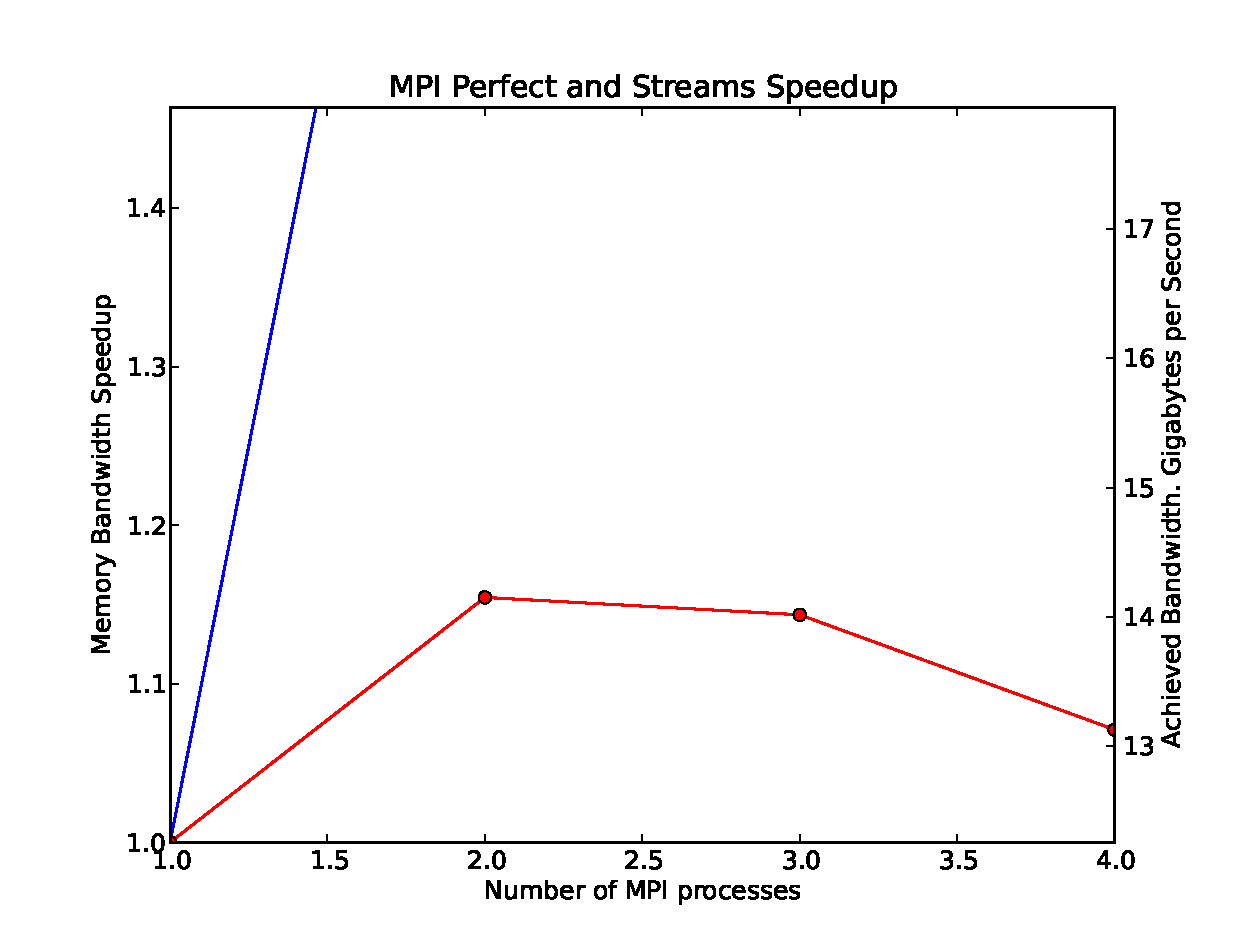
\includegraphics[width=.8\textwidth, height=.4\textwidth]{petsc_3_5_4_with_fftw_and_complex_number_configuration.eps}
%     \caption*{PetscScalar: Evaluate the Computer System using Complex Numbers}
%     \label{checkerboard_lattice}
% \end{figure}

%%%%%%%%%%%%%%%%%%%%%%%%%%%%%%%%%%%%%%%%%%%%%%%%%%%%%%%%%%%%%%%%%%%%%%%%%%%%%%%%
                        % Concluding Pages %
%%%%%%%%%%%%%%%%%%%%%%%%%%%%%%%%%%%%%%%%%%%%%%%%%%%%%%%%%%%%%%%%%%%%%%%%%%%%%%%%



%%%%%%%%%%%%%%%%%%%%%%%%%%%%%%%%%%%%%%%%%%%%%%%%%%%%%%%%%%%%%%%%%%%%%%%%%%%%%%%%
                             % Appendices Pages %
%%%%%%%%%%%%%%%%%%%%%%%%%%%%%%%%%%%%%%%%%%%%%%%%%%%%%%%%%%%%%%%%%%%%%%%%%%%%%%%%

% \appendix
% \section{Appendices}
% \subsection{First appendix}
% \subsection{Second appendix}

\appendix
\addcontentsline{toc}{section}{Appendices}
\section*{Appendices}
\section{First appendix}
\section{Second appendix}


%%%%%%%%%%%%%%%%%%%%%%%%%%%%%%%%%%%%%%%%%%%%%%%%%%%%%%%%%%%%%%%%%%%%%%%%%%%%%%%%
                           %  Bibliography Pages %
%%%%%%%%%%%%%%%%%%%%%%%%%%%%%%%%%%%%%%%%%%%%%%%%%%%%%%%%%%%%%%%%%%%%%%%%%%%%%%%%

% Bibliography or References, REQUIRED

% If using bibtex, create or modify the refs.bib file
% and use (uncomment) the following three lines.
%\bibliographystyle{plain}     %You may prefer \bibliographystyle{alpha}
%\addcontentsline{toc}{chapter}{\bibname}
%\bibliography{refs}         

% If using the ``thereference'' environment instead, modify the ref.tex file
% and use the following line
%\include{ref}
%\bibliography{Bibliography_HTCondor}
\newpage
\bibliography{References/TOOLS_Bibliography}
\end{document}
